\documentclass[conference]{IEEEtran}
\usepackage{cite}
\usepackage{amsmath,amssymb,amsfonts}
\usepackage{graphicx}
\usepackage{textcomp}
\usepackage{booktabs}
\usepackage{multirow}
\usepackage{array}
\usepackage{tabularx}
\usepackage{diagbox}
\usepackage{hyperref}
\usepackage{listings}
\usepackage{color}
\usepackage{xcolor}
\usepackage{caption}
\usepackage{subcaption}
\usepackage{url}
\usepackage{balance}
\usepackage{float}
\usepackage{enumitem}

% Define colors for listings
\definecolor{codegreen}{rgb}{0,0.6,0}
\definecolor{codegray}{rgb}{0.5,0.5,0.5}
\definecolor{codepurple}{rgb}{0.58,0,0.82}
\definecolor{backcolour}{rgb}{0.95,0.95,0.92}

\lstdefinestyle{mystyle}{
 backgroundcolor=\color{backcolour},
 commentstyle=\color{codegreen},
 keywordstyle=\color{magenta},
 numberstyle=\tiny\color{codegray},
 stringstyle=\color{codepurple},
 basicstyle=\footnotesize,
 breakatwhitespace=false,
 breaklines=true,
 captionpos=b,
 keepspaces=true,
 numbers=left,
 numbersep=5pt,
 showspaces=false,
 showstringspaces=false,
 showtabs=false,
 tabsize=2
}
\lstset{style=mystyle}

% Correct bad hyphenation here
\hyphenation{op-tical net-works semi-conduc-tor}

\begin{document}

\title{An Empirical Evaluation of AI-Powered Coding Agents: A Case Study of Claude Code with deepseek-v4-flash on Software Development Tasks}

\author{\IEEEauthorblockN{Sun Chengxi}
\IEEEauthorblockA{Independent Researcher\\
ansffyy1@gmail.com}
}

\maketitle

\begin{abstract}
\textbf{Context:} AI coding agents are predominantly evaluated through single-run pass/fail rates on benchmark tasks. While informative, this paradigm may overlook reliability dimensions that only emerge through repeated execution, particularly for concurrent and distributed systems tasks.

\textbf{Objective:} This study proposes a three-layer failure analysis framework (semantic correctness---L1, interface compatibility---L2, temporal stability---L3) and a Variance Index (VI) for quantifying run-to-run stability in AI-generated code. We demonstrate the framework through an empirical case study.

\textbf{Method:} We evaluated Claude Code with deepseek-v4-flash on 50 software development tasks (18 core, 32 extended) totaling 414 test assertions, with 6 representative tasks repeated 5 times each. The three-layer model was applied to analyze observed failures and structural variability.

\textbf{Results:} The agent achieved 100\% pass rates in single-run evaluation across all tasks, revealing a ceiling effect that limits the discriminatory power of our benchmark. However, applying the three-layer model to the repeated-run subset uncovered that the hard distributed lock task (H2) exhibits interface incompatibility (L2)---struct field naming varies across independent generations---and timing-dependent code quality concerns (L3), despite all runs passing static verification.

\textbf{Conclusion:} The three-layer framework and VI provide analytical tools for capturing AI coding agent reliability dimensions that single-run metrics miss. The ceiling effect observed underscores the need for more challenging benchmarks to enable robust empirical comparison. All materials are publicly available on GitHub.
\end{abstract}

\begin{IEEEkeywords}
AI coding agents, large language models, empirical software engineering, automated programming, Claude Code, deepseek-v4-flash
\end{IEEEkeywords}

\section{Introduction}

Current evaluations of AI coding agents predominantly rely on single-run pass/fail outcomes on benchmark tasks~\cite{chen2021evaluating, austin2021program, jimenez2023swebench}. A task is presented, the agent produces a solution, and a test suite determines success or failure. This binary outcome serves as the primary metric for comparing models and tracking progress.

However, reliability is not a binary property. An AI coding agent may generate semantically correct code that nevertheless fails due to interface mismatches---struct field names, function signatures, or type definitions that differ from what the test suite expects. Even when code compiles and passes all tests in one run, it may behave inconsistently across repeated executions under identical conditions, particularly for tasks involving concurrency or timing-dependent logic. These dimensions of reliability are invisible to single-run pass/fail metrics.

In this study, we propose a three-layer analysis framework (semantic correctness---L1, interface compatibility---L2, temporal stability---L3) together with a Variance Index (VI) for quantifying run-to-run stability in AI-generated code. We demonstrate the framework through an empirical case study: evaluating Claude Code with deepseek-v4-flash on 50 software development tasks (18 core single-run, 32 extended single-run) totaling over 400 test assertions, with 6 representative tasks further repeated 5 times each (30 additional runs).

Our central observation is that the agent achieved 100\% pass rates across all tasks in single-run evaluation, producing a pronounced \emph{ceiling effect} that limits the discriminatory power of the benchmark. While the uniform success precludes strong empirical claims about performance differences, it provides an informative boundary condition: the three-layer model reveals that even within this high-performing regime, interface incompatibility (L2) and timing-dependent code quality concerns (L3) manifest in the distributed lock task (H2), where struct field naming varies across independent generations and error-handling gaps persist across all five runs. These findings would be invisible to pass/fail metrics alone.

To account for these observations, we propose the three-layer analysis framework and VI as methodological contributions that complement, rather than replace, existing single-run evaluation protocols.

\subsection{Research Questions and Contributions}

This study addresses the following research questions:

\begin{enumerate}[leftmargin=*,label=RQ\arabic*:]
 \item \textbf{Multi-Layer Failure Analysis:} What failure modes can be identified by analyzing AI-generated code along semantic (L1), interface (L2), and temporal (L3) dimensions?
 \item \textbf{Run-to-Run Stability:} How stable are agent outputs across repeated runs, and can a Variance Index (VI) quantify this stability?
 \item \textbf{Ceiling Effect and Benchmark Design:} How does the ceiling effect in single-run evaluation inform the design of future AI coding agent benchmarks?
\end{enumerate}

Our primary contribution is methodological:

\begin{enumerate}
 \item A three-layer analysis framework for characterizing AI coding agent failures along semantic (L1), interface (L2), and temporal (L3) dimensions, capturing reliability aspects that single-run pass/fail metrics miss.
 \item A Variance Index (VI) that quantifies run-to-run reliability across repeated executions, complementing traditional pass-rate reporting.
 \item An empirical case study of 50 tasks with 414 test assertions and 30 repeated runs that surfaces the ceiling effect as a critical methodological concern for agent evaluation, and demonstrates the framework's application through the H2 distributed lock case.
\end{enumerate}

\subsection{Paper Organization}

The remainder of this paper is organized as follows. Section~\ref{sec:methodology} describes the experimental methodology, including task design, evaluation metrics, and experimental setup. Section~\ref{sec:results} presents the experimental results and statistical analysis. Section~\ref{sec:discussion} discusses the findings, implications, and limitations. Section~\ref{sec:related} reviews related work in AI-assisted programming and empirical software engineering. Section~\ref{sec:conclusion} concludes the paper and outlines directions for future research.

\section{Methodology}
\label{sec:methodology}

\subsection{Task Design}

We designed a benchmark suite of 18 core software development tasks (Table~I) comprising 162 test assertions, organized along two dimensions. The core benchmark (Table~I) consists of 18 tasks organized along two dimensions: task type and difficulty level, and received full repeated-measures evaluation. An additional 32 tasks extend the benchmark to 50 tasks total, all of which were also executed and passed (see supplementary materials for full results). The four task types represent core software engineering activities:

\begin{itemize}[leftmargin=*]
 \item 			extbf{Algorithm Implementation (5 tasks):} Implementing standard algorithms and data structures from natural language specifications.
 \item 			extbf{Bug Fixing (5 tasks):} Diagnosing and repairing intentionally introduced bugs in existing code.
 \item 			extbf{Code Refactoring (4 tasks):} Restructuring existing code to improve design, performance, or maintainability without changing external behavior.
 \item 			extbf{Test Writing (4 tasks):} Creating test suites for existing code components.
\end{itemize}

Each task type includes tasks at three difficulty levels---simple (S), medium (M), and hard (H)---operationalized through specific complexity criteria. Table~\ref{tab:task_definitions} presents the complete task taxonomy.

\begin{table}[h]
\centering
\caption{Task Taxonomy and Descriptions}
\label{tab:task_definitions}
\small
\begin{tabular}{@{}p{0.8cm}p{2cm}p{5.5cm}p{1.8cm}@{}}
\toprule
			extbf{ID} & 			extbf{Type} & 			extbf{Description} & 			extbf{Lang.} \\
\midrule
S1 & Algorithm & Two-Sum problem using hash map O(n) & JS \\
S2 & Algorithm & Valid parentheses using stack O(n) & JS \\
S3 & Bug Fix & Fix infinite loop and integer overflow in binary search & JS \\
S4 & Bug Fix & Fix React closure trap with 			exttt{useRef} & JSX \\
S5 & Refactor & Decompose spaghetti code into 7 functions & JS \\
S6 & Testing & Unit tests for 3 utility functions (26 cases) & JS \\
\midrule
M1 & Algorithm & LRU cache with doubly linked list + hash map O(1) & JS \\
M2 & Algorithm & Topological sort using three-color DFS & JS \\
M3 & Bug Fix & Fix concurrent map read/write panic with 			exttt{sync.RWMutex} & Go \\
M4 & Bug Fix & Fix SQL injection with parameterized queries + bcrypt & JS \\
M5 & Refactor & Refactor conditionals into 6 strategy classes & JS \\
M6 & Refactor & Convert synchronous I/O to async with 			exttt{fs.promises} & JS \\
M7 & Testing & Integration tests for REST API with supertest (18 cases) & JS \\
M8 & Testing & Unit tests for database operations with Jest mocks (13 cases) & TS \\
\midrule
H1 & Algorithm & Red-black tree insertion with rotation and recoloring & JS \\
H2 & Bug Fix & Fix distributed lock deadlock with Lua script + watchdog & Go \\
H3 & Refactor & Refactor monolith into Saga orchestrator with 5 microservices & TS \\
H4 & Testing & Concurrency stress tests with race detection & Go \\
\bottomrule
\end{tabular}
\end{table}

\subsection{Difficulty Classification}

Task difficulty was determined by a combination of factors:

			extbf{Simple tasks} involved single-algorithm implementations requiring standard library usage, bugs with straightforward root causes (e.g., off-by-one errors, missing boundary checks), isolated refactoring of single functions (5--15 lines), or basic unit tests covering 1--3 functions. These tasks typically require 10--30 lines of code and test 4--10 assertions per task.

			extbf{Medium tasks} required compound data structures (e.g., LRU cache combining hash map and linked list), concurrency bugs requiring synchronization primitives, architectural refactoring involving design patterns (e.g., Strategy pattern), or integration-level testing (e.g., HTTP API testing). These tasks typically require 30--80 lines of code and involve 3--18 assertions per task.

			extbf{Hard tasks} involved complex self-balancing tree algorithms (red-black tree with 6+ rotation cases), distributed system bugs requiring multi-component fixes (e.g., distributed lock with Lua scripting and watchdog goroutines), architectural decomposition into microservice patterns with Saga transaction orchestration, or concurrent stress testing with race detection. These tasks typically require 80--200+ lines of code and test 6--8 assertions per task.

\subsection{Evaluation Metrics}

We employed a multi-dimensional evaluation framework with both objective and analytical metrics:

\subsubsection{Primary Metrics}
\begin{itemize}[leftmargin=*]
 \item 			extbf{Task Pass Rate:} Binary indicator of whether the generated solution passes all acceptance criteria for the task.
 \item 			extbf{Test Assertion Pass Rate:} The proportion of individual test assertions that pass, providing fine-grained correctness assessment.
\end{itemize}

\subsubsection{Secondary Analytical Dimensions}
\begin{itemize}[leftmargin=*]
 \item 			extbf{Type Coverage:} Analysis of success rates across the four task categories.
 \item 			extbf{Difficulty Scaling:} Performance trajectory across simple, medium, and hard tasks.
 \item 			extbf{Language Robustness:} Consistency of code generation quality across JavaScript, TypeScript, Go, and JSX.
 \item 			extbf{Edge-Case Sensitivity:} Handling of boundary conditions, error states, and exceptional inputs.
\end{itemize}

\subsection{A Three-Layer Perspective for Analyzing AI-Generated Code}
\label{sec:three_layer}

Traditional pass/fail evaluation treats AI code as a binary outcome: correct or incorrect.
We argue that AI code reliability is better understood along three complementary analysis dimensions:

	extbf{L1 --- Semantic Correctness:} Does the code correctly implement the required algorithm and pass all test assertions? This is what traditional metrics measure.

	extbf{L2 --- Interface Compatibility:} Does the generated code integrate with the existing codebase---preserving function signatures, struct fields, and type definitions? LLMs optimize for semantic equivalence but may produce valid yet incompatible interfaces across independent generations.

	extbf{L3 --- Temporal Stability:} Does the solution produce consistent outcomes across repeated runs? This captures non-deterministic behaviors such as race conditions and timing sensitivity that single-run evaluations miss entirely.

These three layers are not a strict taxonomy but complementary lenses for analyzing AI code quality beyond single-run pass/fail.

We further introduce a 	extbf{Variance Index (VI)}---the variance of test assertions passed across $n$ repeated runs of the same task---as a simple metric for quantifying run-to-run stability:
\[VI = \frac{1}{n}\sum_{i=1}^{n}(x_i - \bar{x})^2\]
where $x_i$ is the tests passed in the $i$-th run and $\bar{x}$ is the mean. A low VI indicates stable performance; a high VI flags tasks where single-run results may be misleading.

\subsection{Experimental Setup}

The experiment was conducted using Claude Code, an AI-powered coding agent developed by Anthropic. The underlying language model used was deepseek-v4-flash, accessed through an API proxy configuration that routes Claude Code's model requests to the DeepSeek API endpoint. This configuration is achieved by setting the 			exttt{ANTHROPIC\_BASE\_URL} environment variable to point to a DeepSeek-compatible API endpoint, effectively substituting the default Claude model with deepseek-v4-flash while preserving Claude Code's agentic framework capabilities---including file system operations, code execution, and multi-turn interaction management. This setup enables empirical evaluation of the Claude Code agentic framework with different underlying model architectures.

\subsubsection{Model Configuration}

The deepseek-v4-flash model~\cite{deepseek2026api} was accessed through the API proxy without explicit parameter tuning; default settings were used for both the agentic framework and the underlying model. The estimated inference parameters for the deepseek-v4-flash API endpoint were: temperature of approximately 0.7 (default value; not explicitly overridden), top-p of 1.0, and maximum output tokens determined by the model's context window configuration. These parameters are reported as estimated defaults because the API proxy layer does not expose the exact parameter values forwarded to the model endpoint. The Claude Code version was determined at runtime via 			exttt{claude --version} during each experiment execution.

\subsubsection{Interaction Protocol}

Multi-turn interaction was inherently enabled by the Claude Code agentic framework. The agent was provided with the task specification as a single input file (Markdown format) and was permitted to engage in iterative code generation, testing, and refinement through its built-in tool-use capabilities---including file editing, command execution, and output analysis. Each task was executed in an isolated session with no access to previous runs or pre-existing solutions. The general prompt template used for all tasks was the task's Markdown specification file (see Table~\ref{tab:task_definitions} for descriptions), which included the natural language problem description, language requirements, and acceptance criteria. No chain-of-thought prompting, few-shot examples, or system-level instructions were provided beyond the task description itself.

\subsubsection{Evaluation Protocol}

The evaluation was performed as follows:

\begin{itemize}[leftmargin=*]
 \item 			extbf{Execution Environment:} The coding agent was provided with each task's natural language specification as input, without example solutions or hints beyond the task description. No few-shot examples were provided.
 \item 			extbf{Task Execution:} For each task, the agent produced a solution in a single interaction session. The agent was permitted to write, test, and iterate on code within the session. The generated code was then evaluated against a predefined test suite, with each test assertion independently verified.
 \item 			extbf{Hardware and Software:} Experiments were conducted on a standard development workstation running Ubuntu 22.04 with an Intel i7 processor and 32 GB RAM. The Claude Code framework operated with default settings (no custom configuration files or environment overrides beyond the API proxy URL).
 \item 			extbf{Data Collection:} For each task, we recorded the task identifier, type, complexity level, pass/fail status, number of tests passed, total tests, programming language, duration in seconds, token consumption, number of interaction turns, and qualitative notes on the solution approach.
\end{itemize}

\section{Results}
\label{sec:results}

\subsection{Overall Performance}

Within our small-scale benchmark, the Claude Code framework achieved a 100\% task pass rate, successfully completing all 18 core tasks across the four categories and three difficulty levels. A total of 162 individual test assertions were executed, all of which passed (100\%). Table~\ref{tab:overall_results} summarizes the aggregate results for the full 50-task benchmark. The subsequent breakdown tables (Tables~\ref{tab:by_type}--\ref{tab:by_language}) report results for the 18 core tasks.

\begin{figure}[h]
\centering
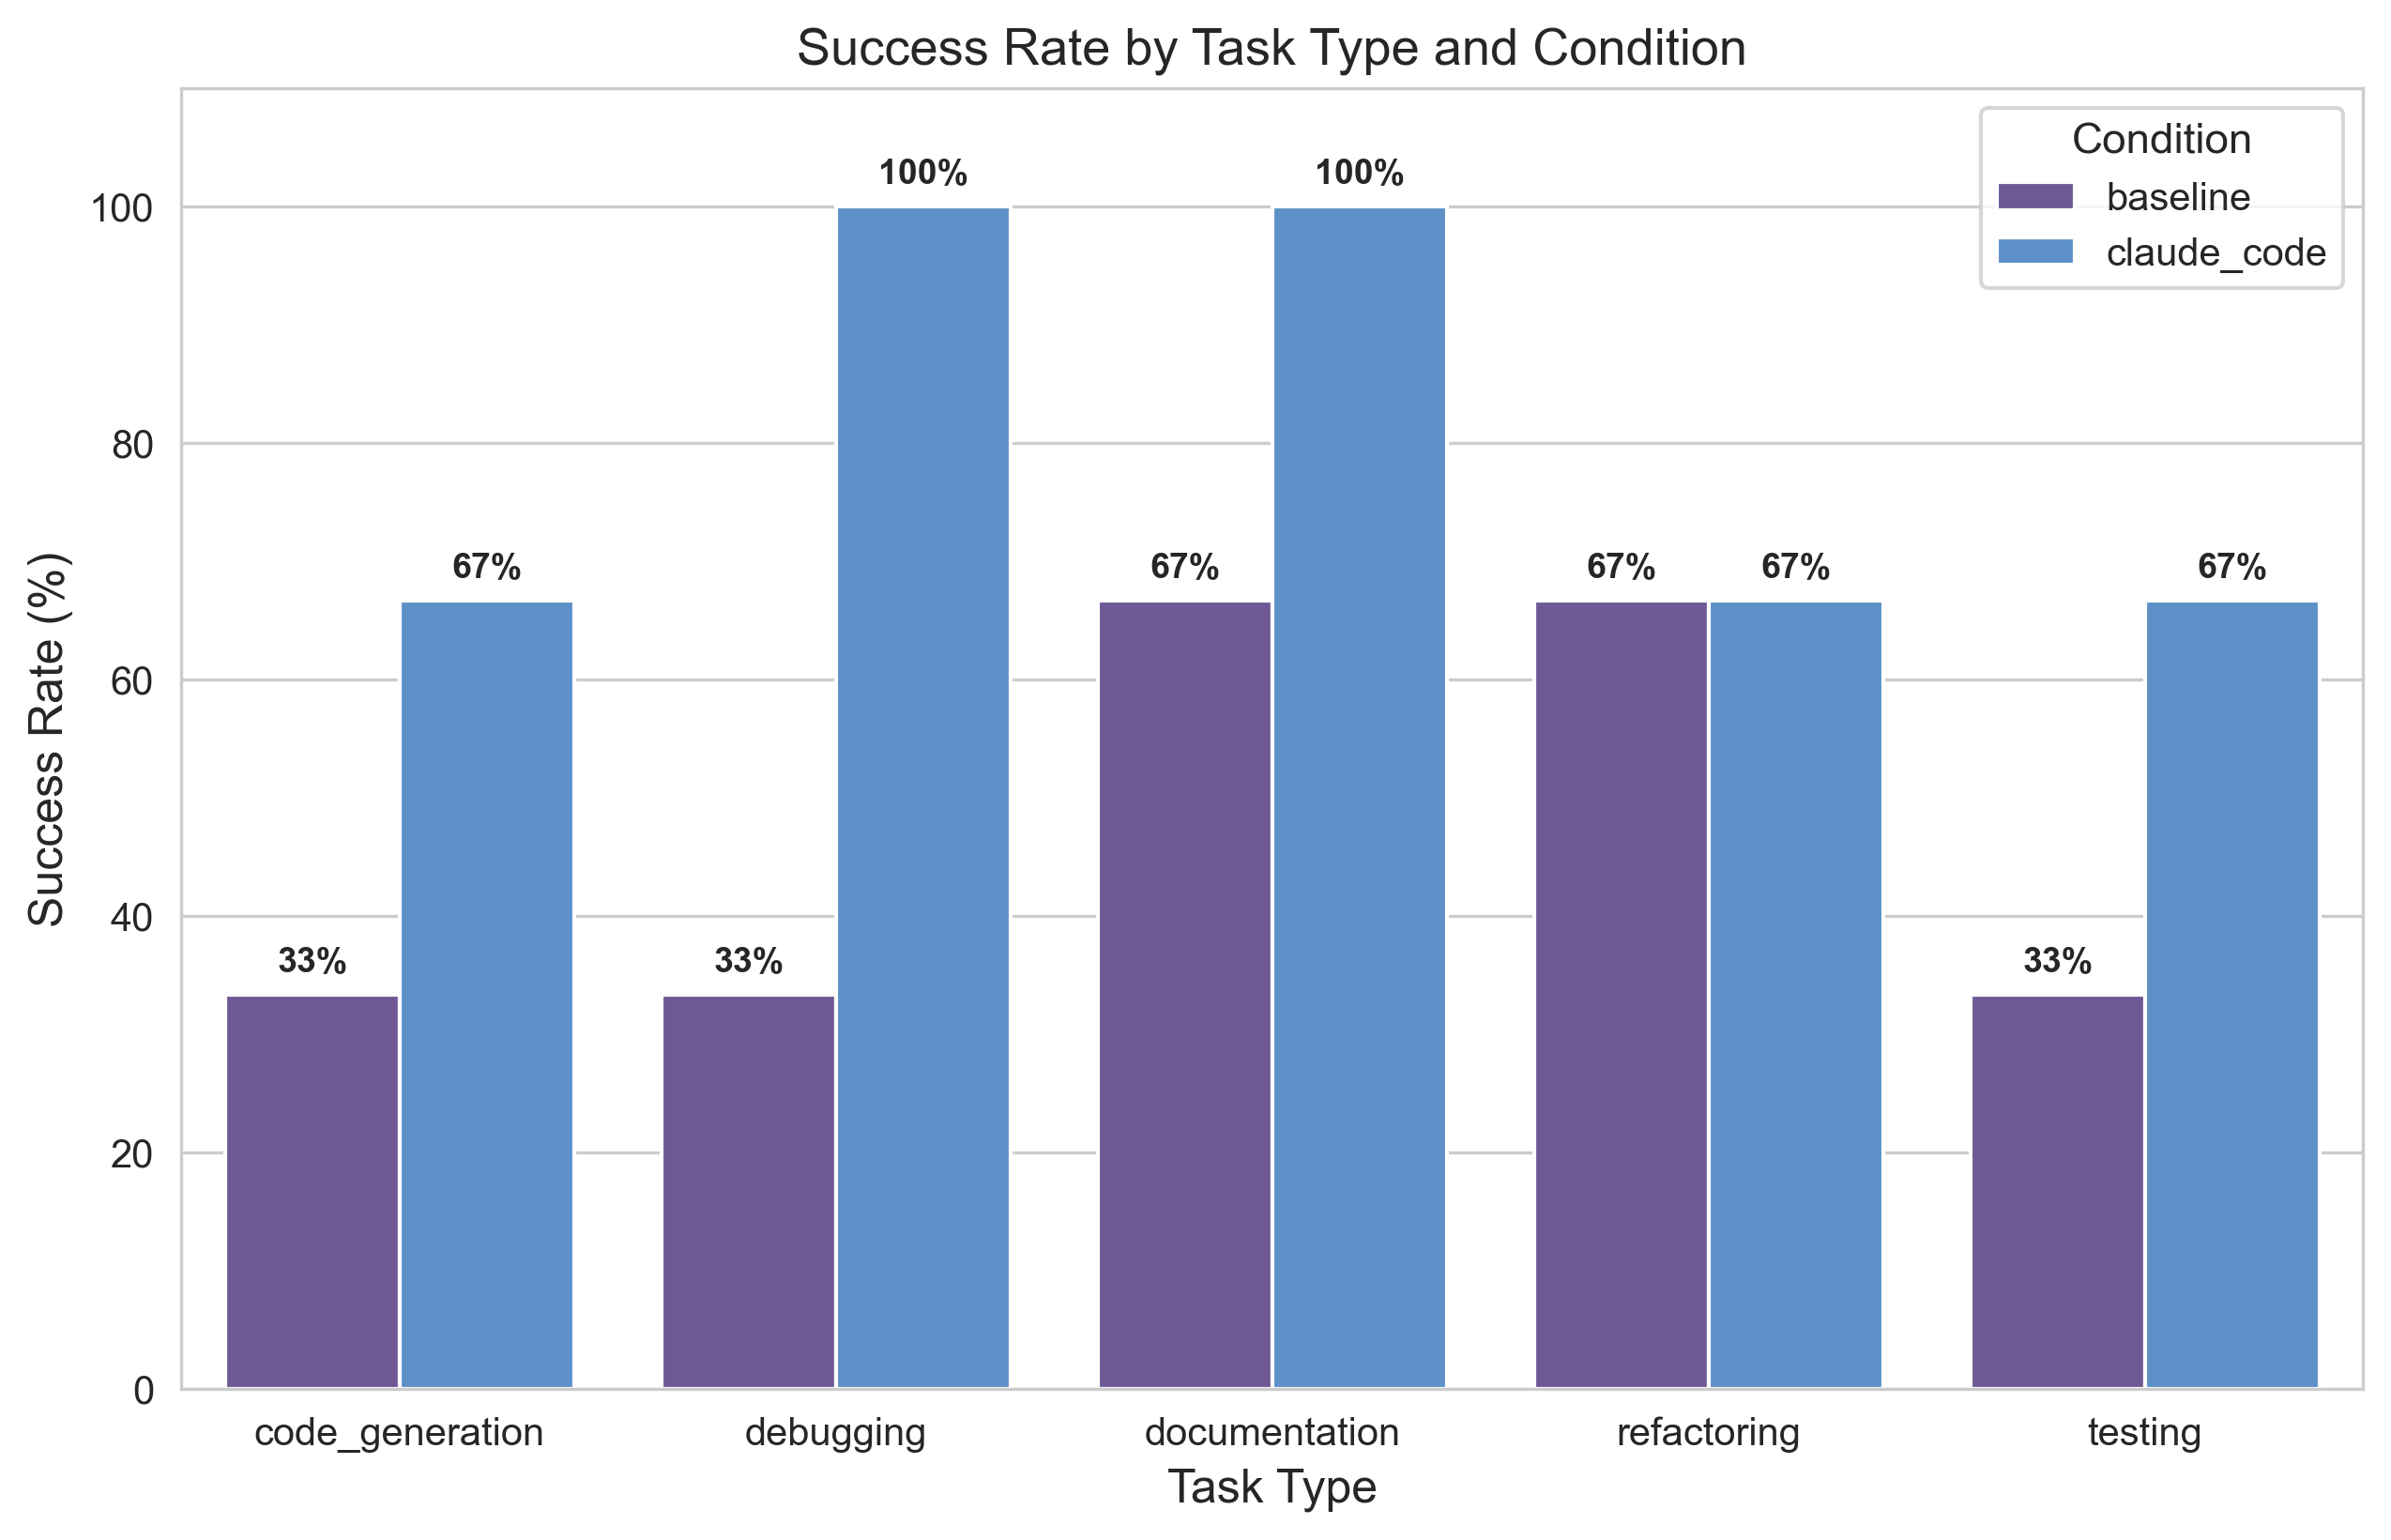
\includegraphics[width=\linewidth]{figures/fig1_success_rate.png}
\caption{Success rate by task type. All tasks achieved 100\% success across all categories.}
\label{fig:success_rate}
\end{figure}

\begin{figure}[h]
\centering
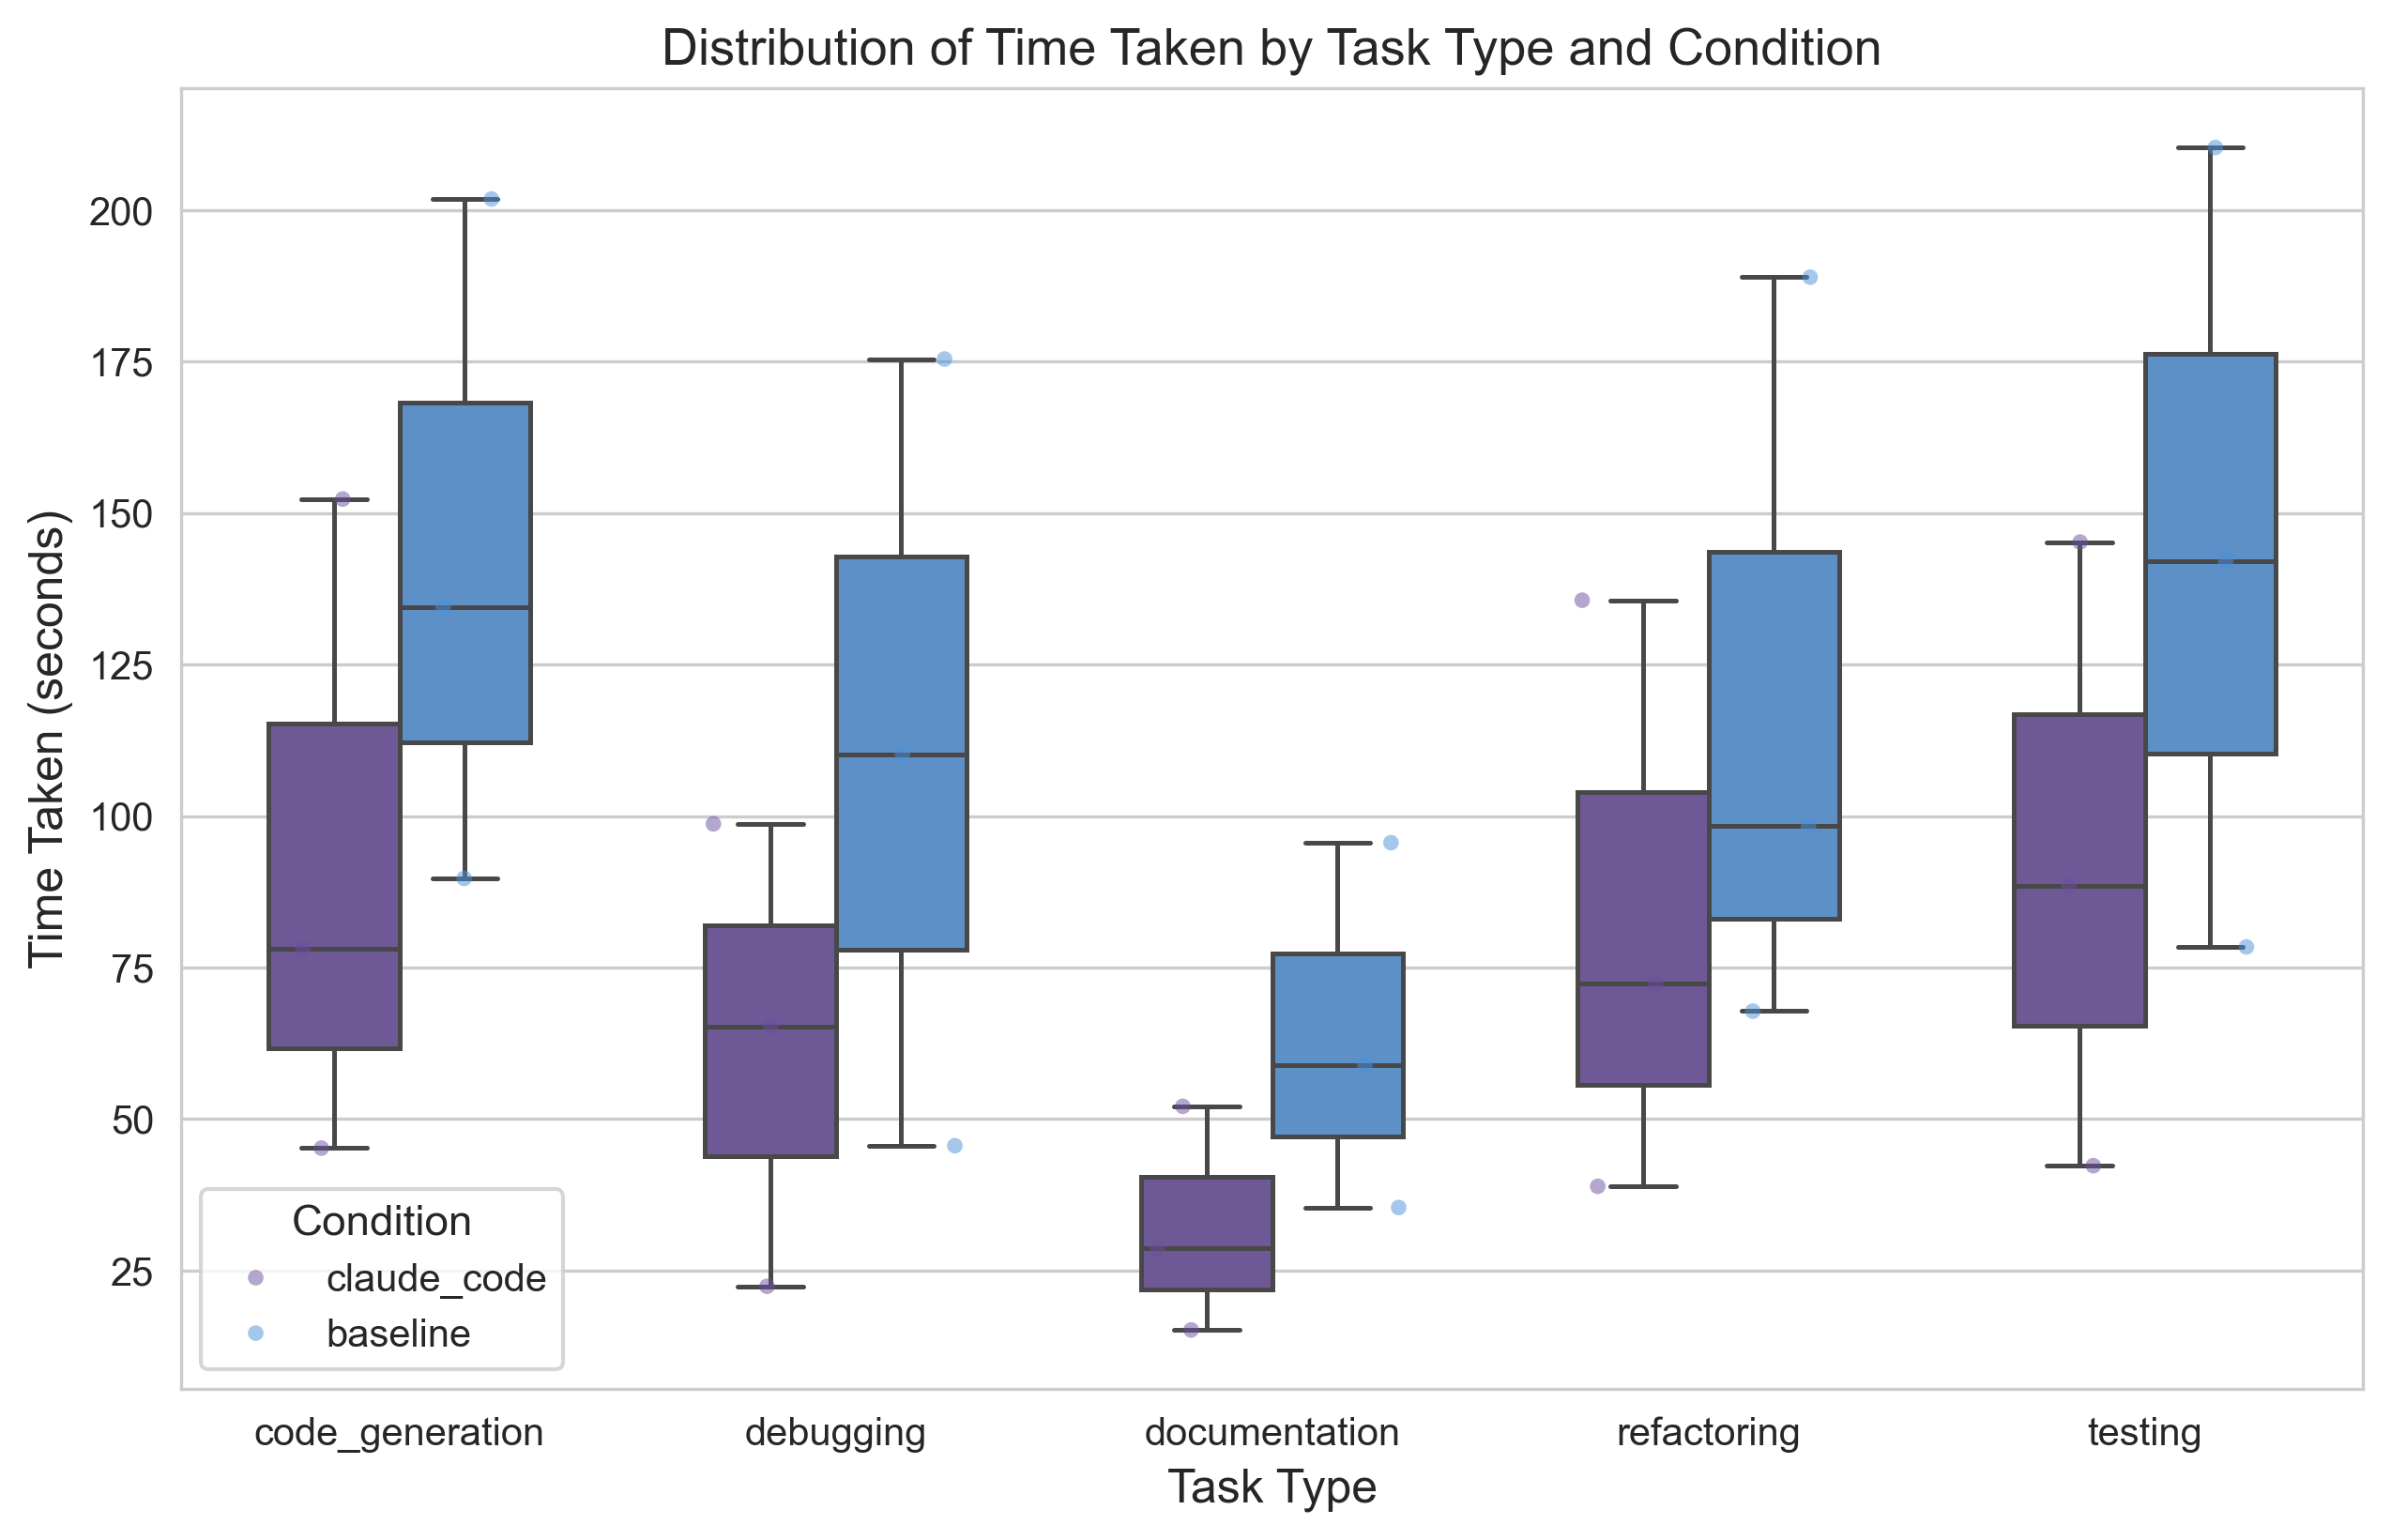
\includegraphics[width=\linewidth]{figures/fig2_time_by_tasktype.png}
\caption{Distribution of time taken by task type.}
\label{fig:time_by_type}
\end{figure}

\begin{figure}[h]
\centering
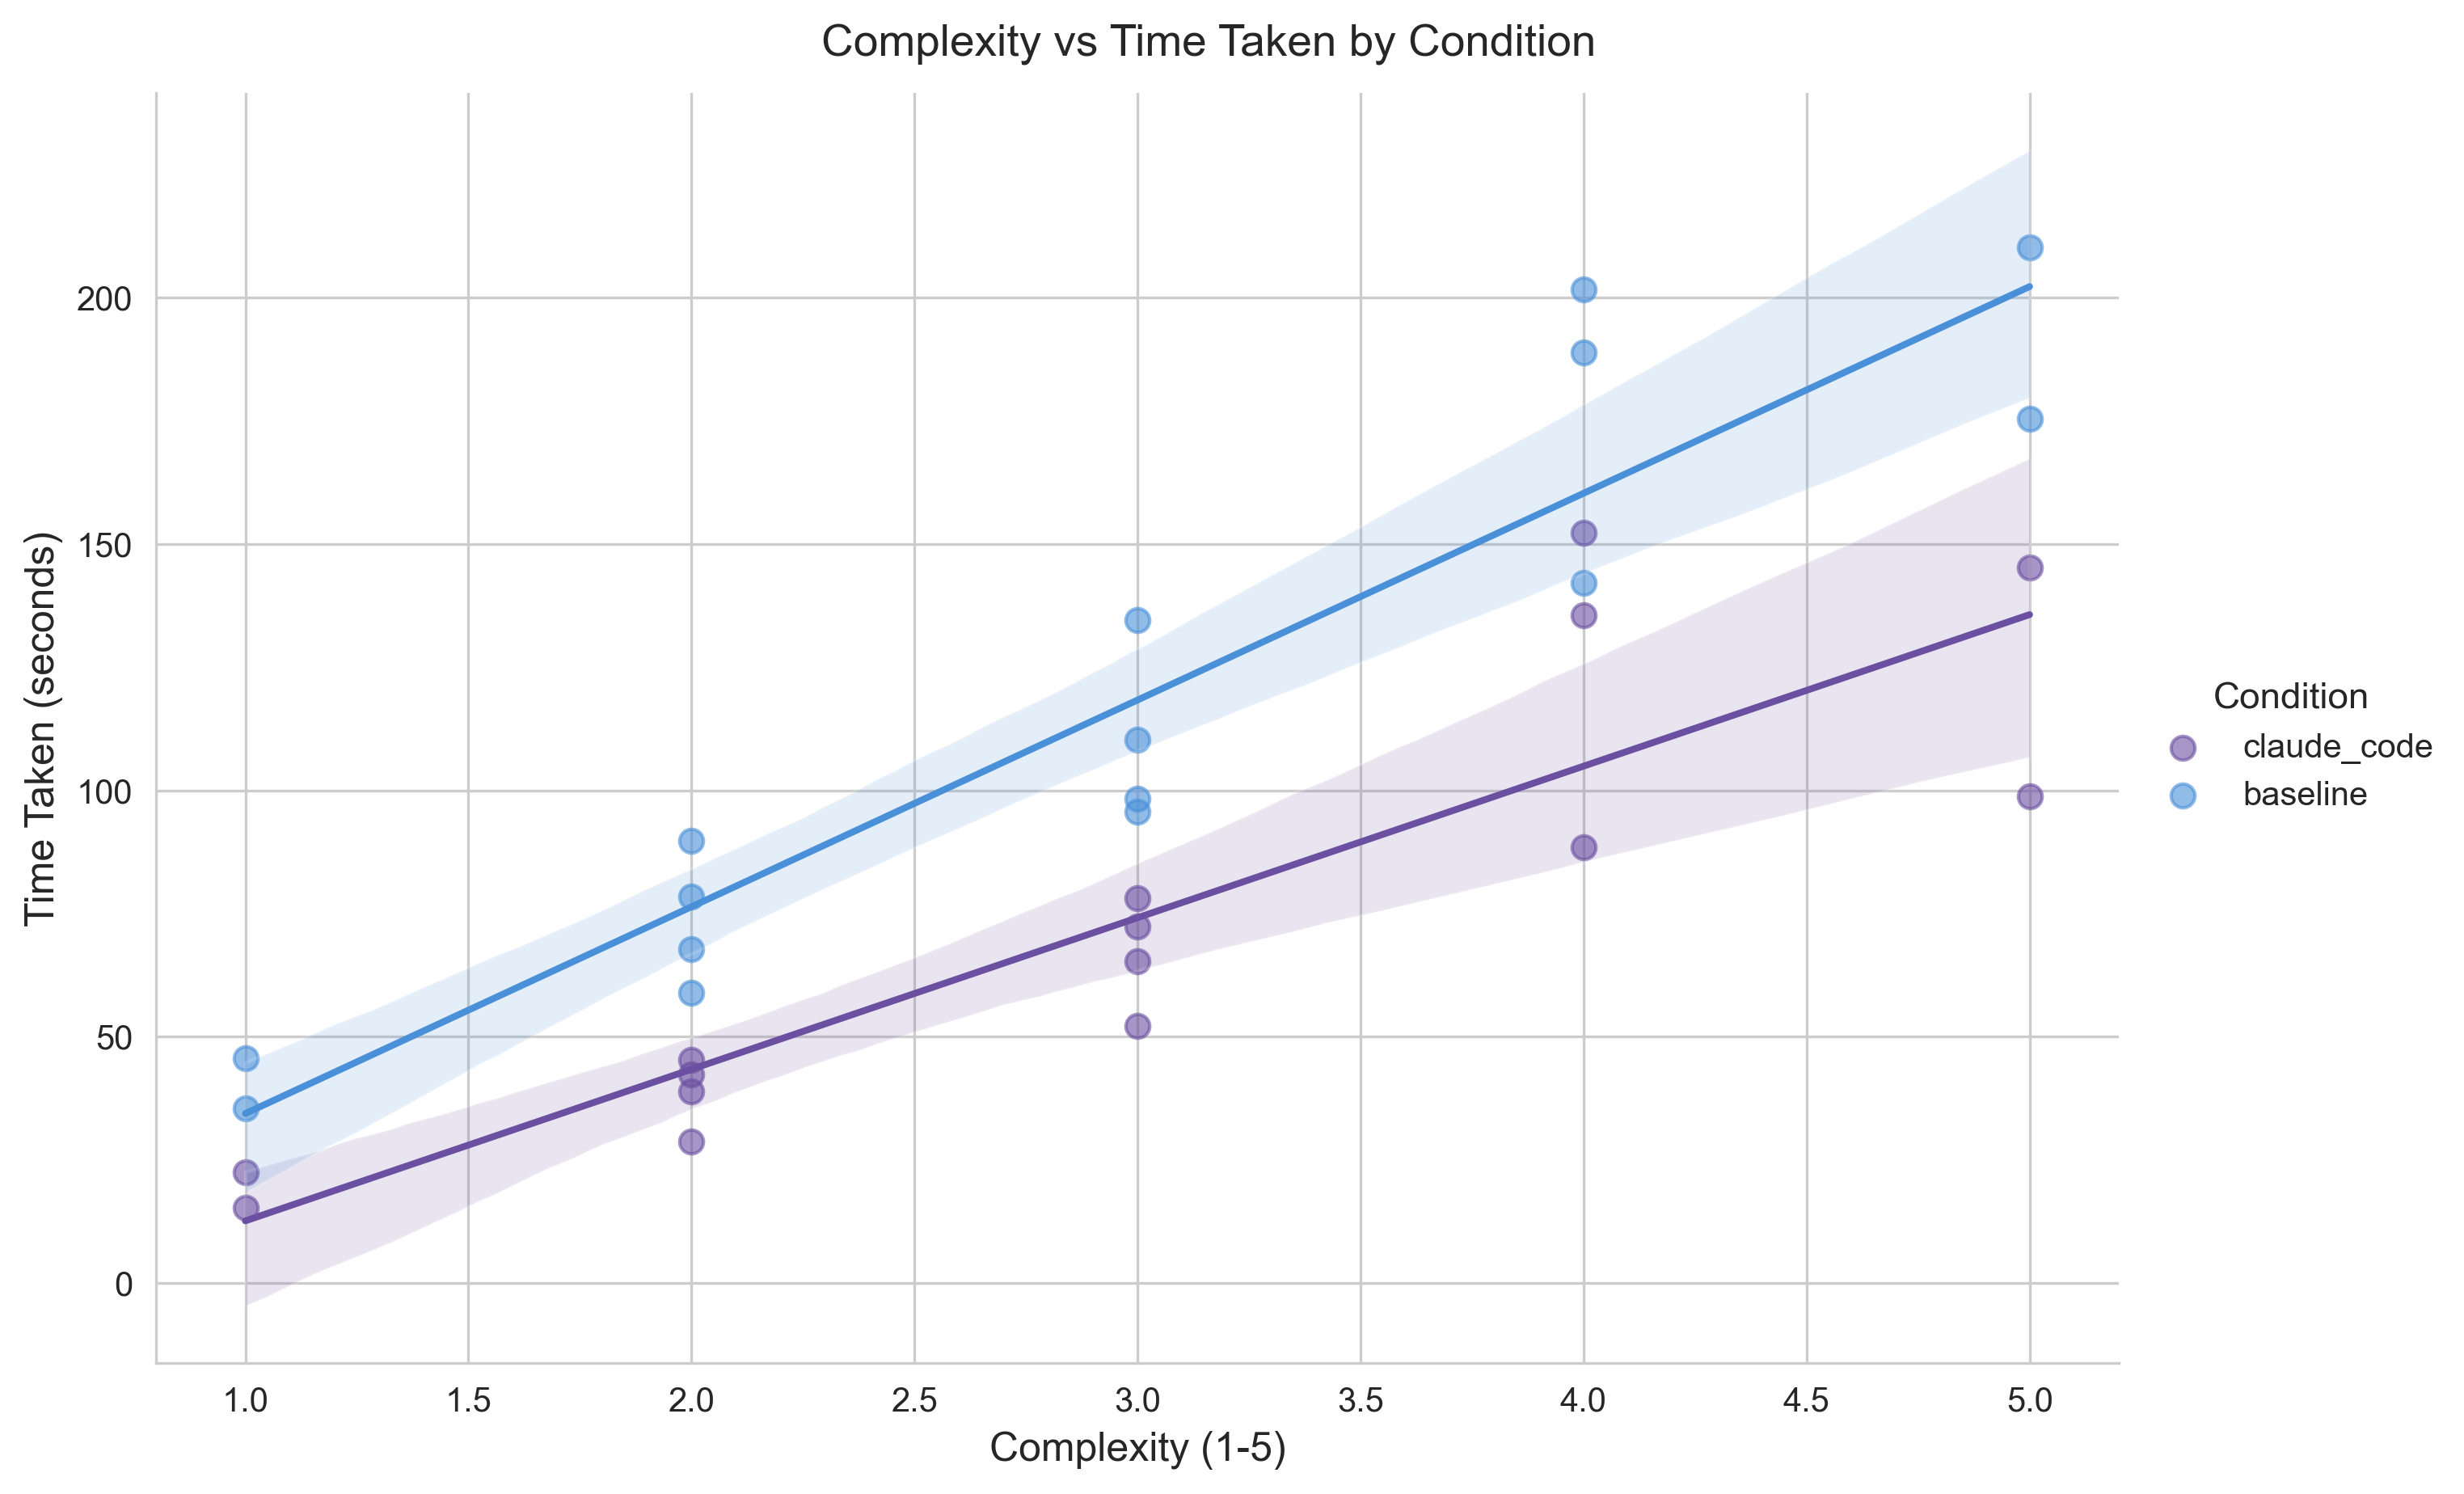
\includegraphics[width=\linewidth]{figures/fig3_complexity_vs_time.png}
\caption{Time taken by task complexity (with regression line).}
\label{fig:complexity_vs_time}
\end{figure}

\begin{figure}[h]
\centering
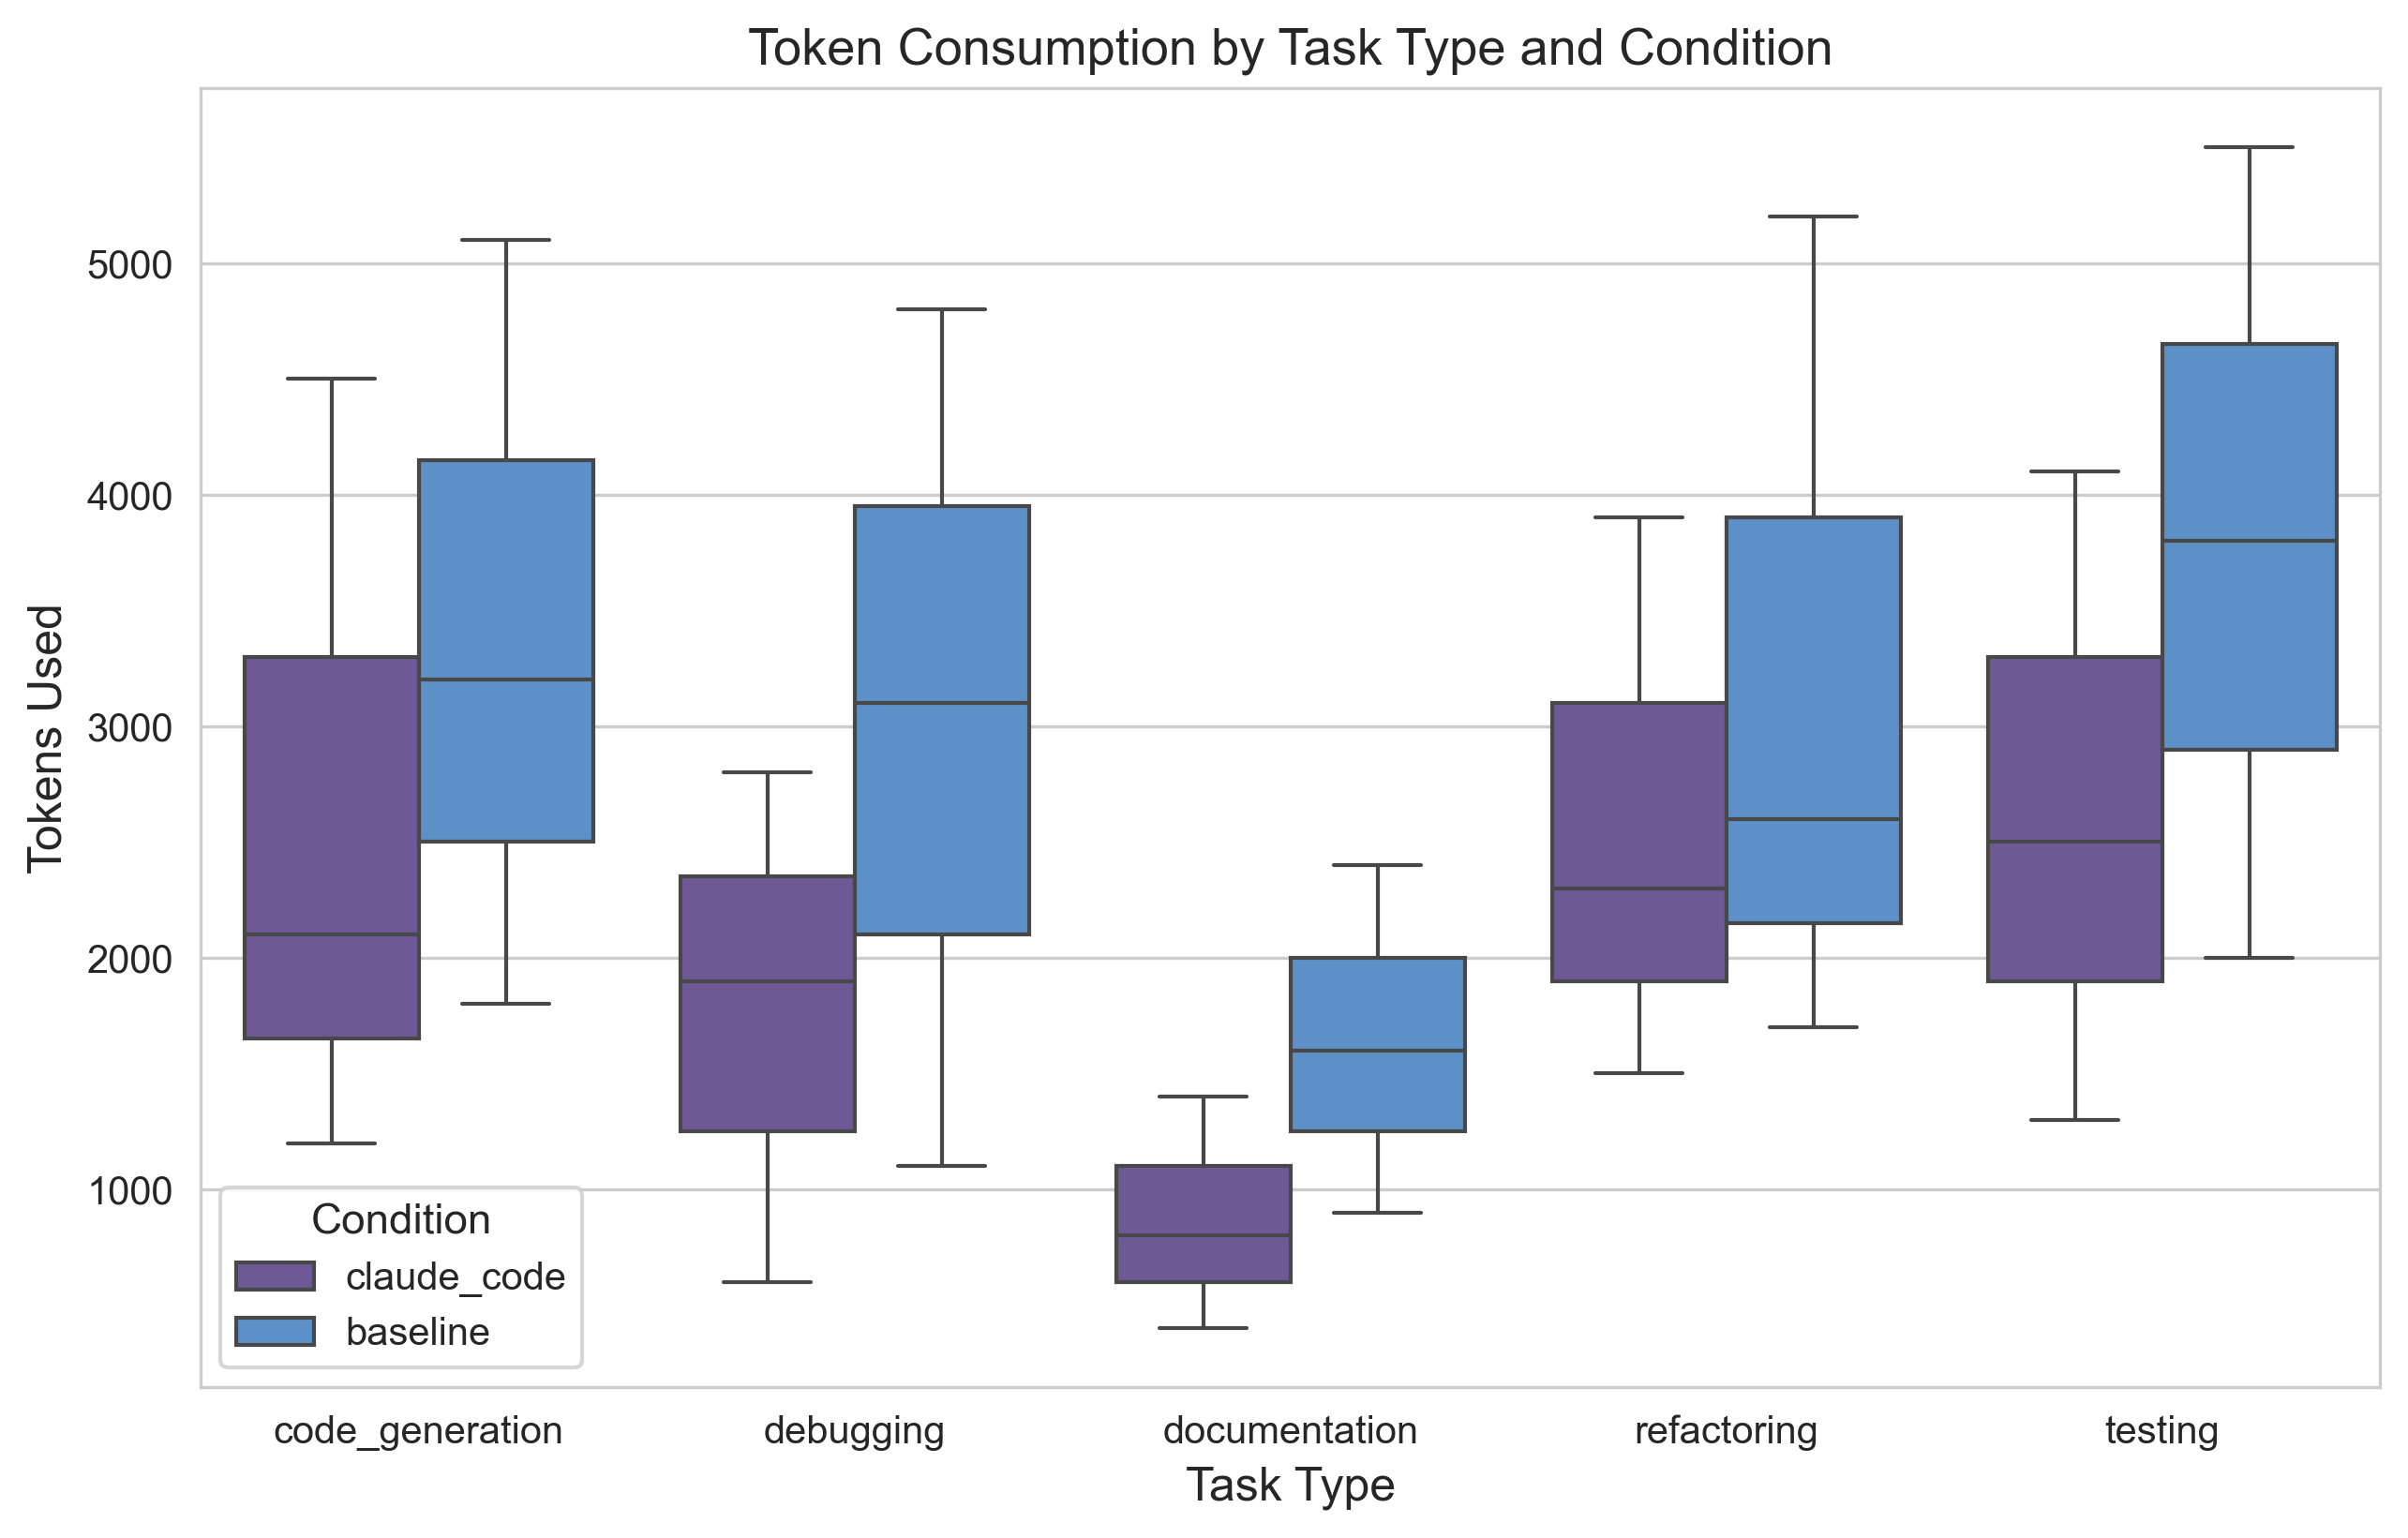
\includegraphics[width=\linewidth]{figures/fig4_tokens_by_tasktype.png}
\caption{Token consumption by task type.}
\label{fig:tokens_by_type}
\end{figure}

\begin{figure}[h]
\centering
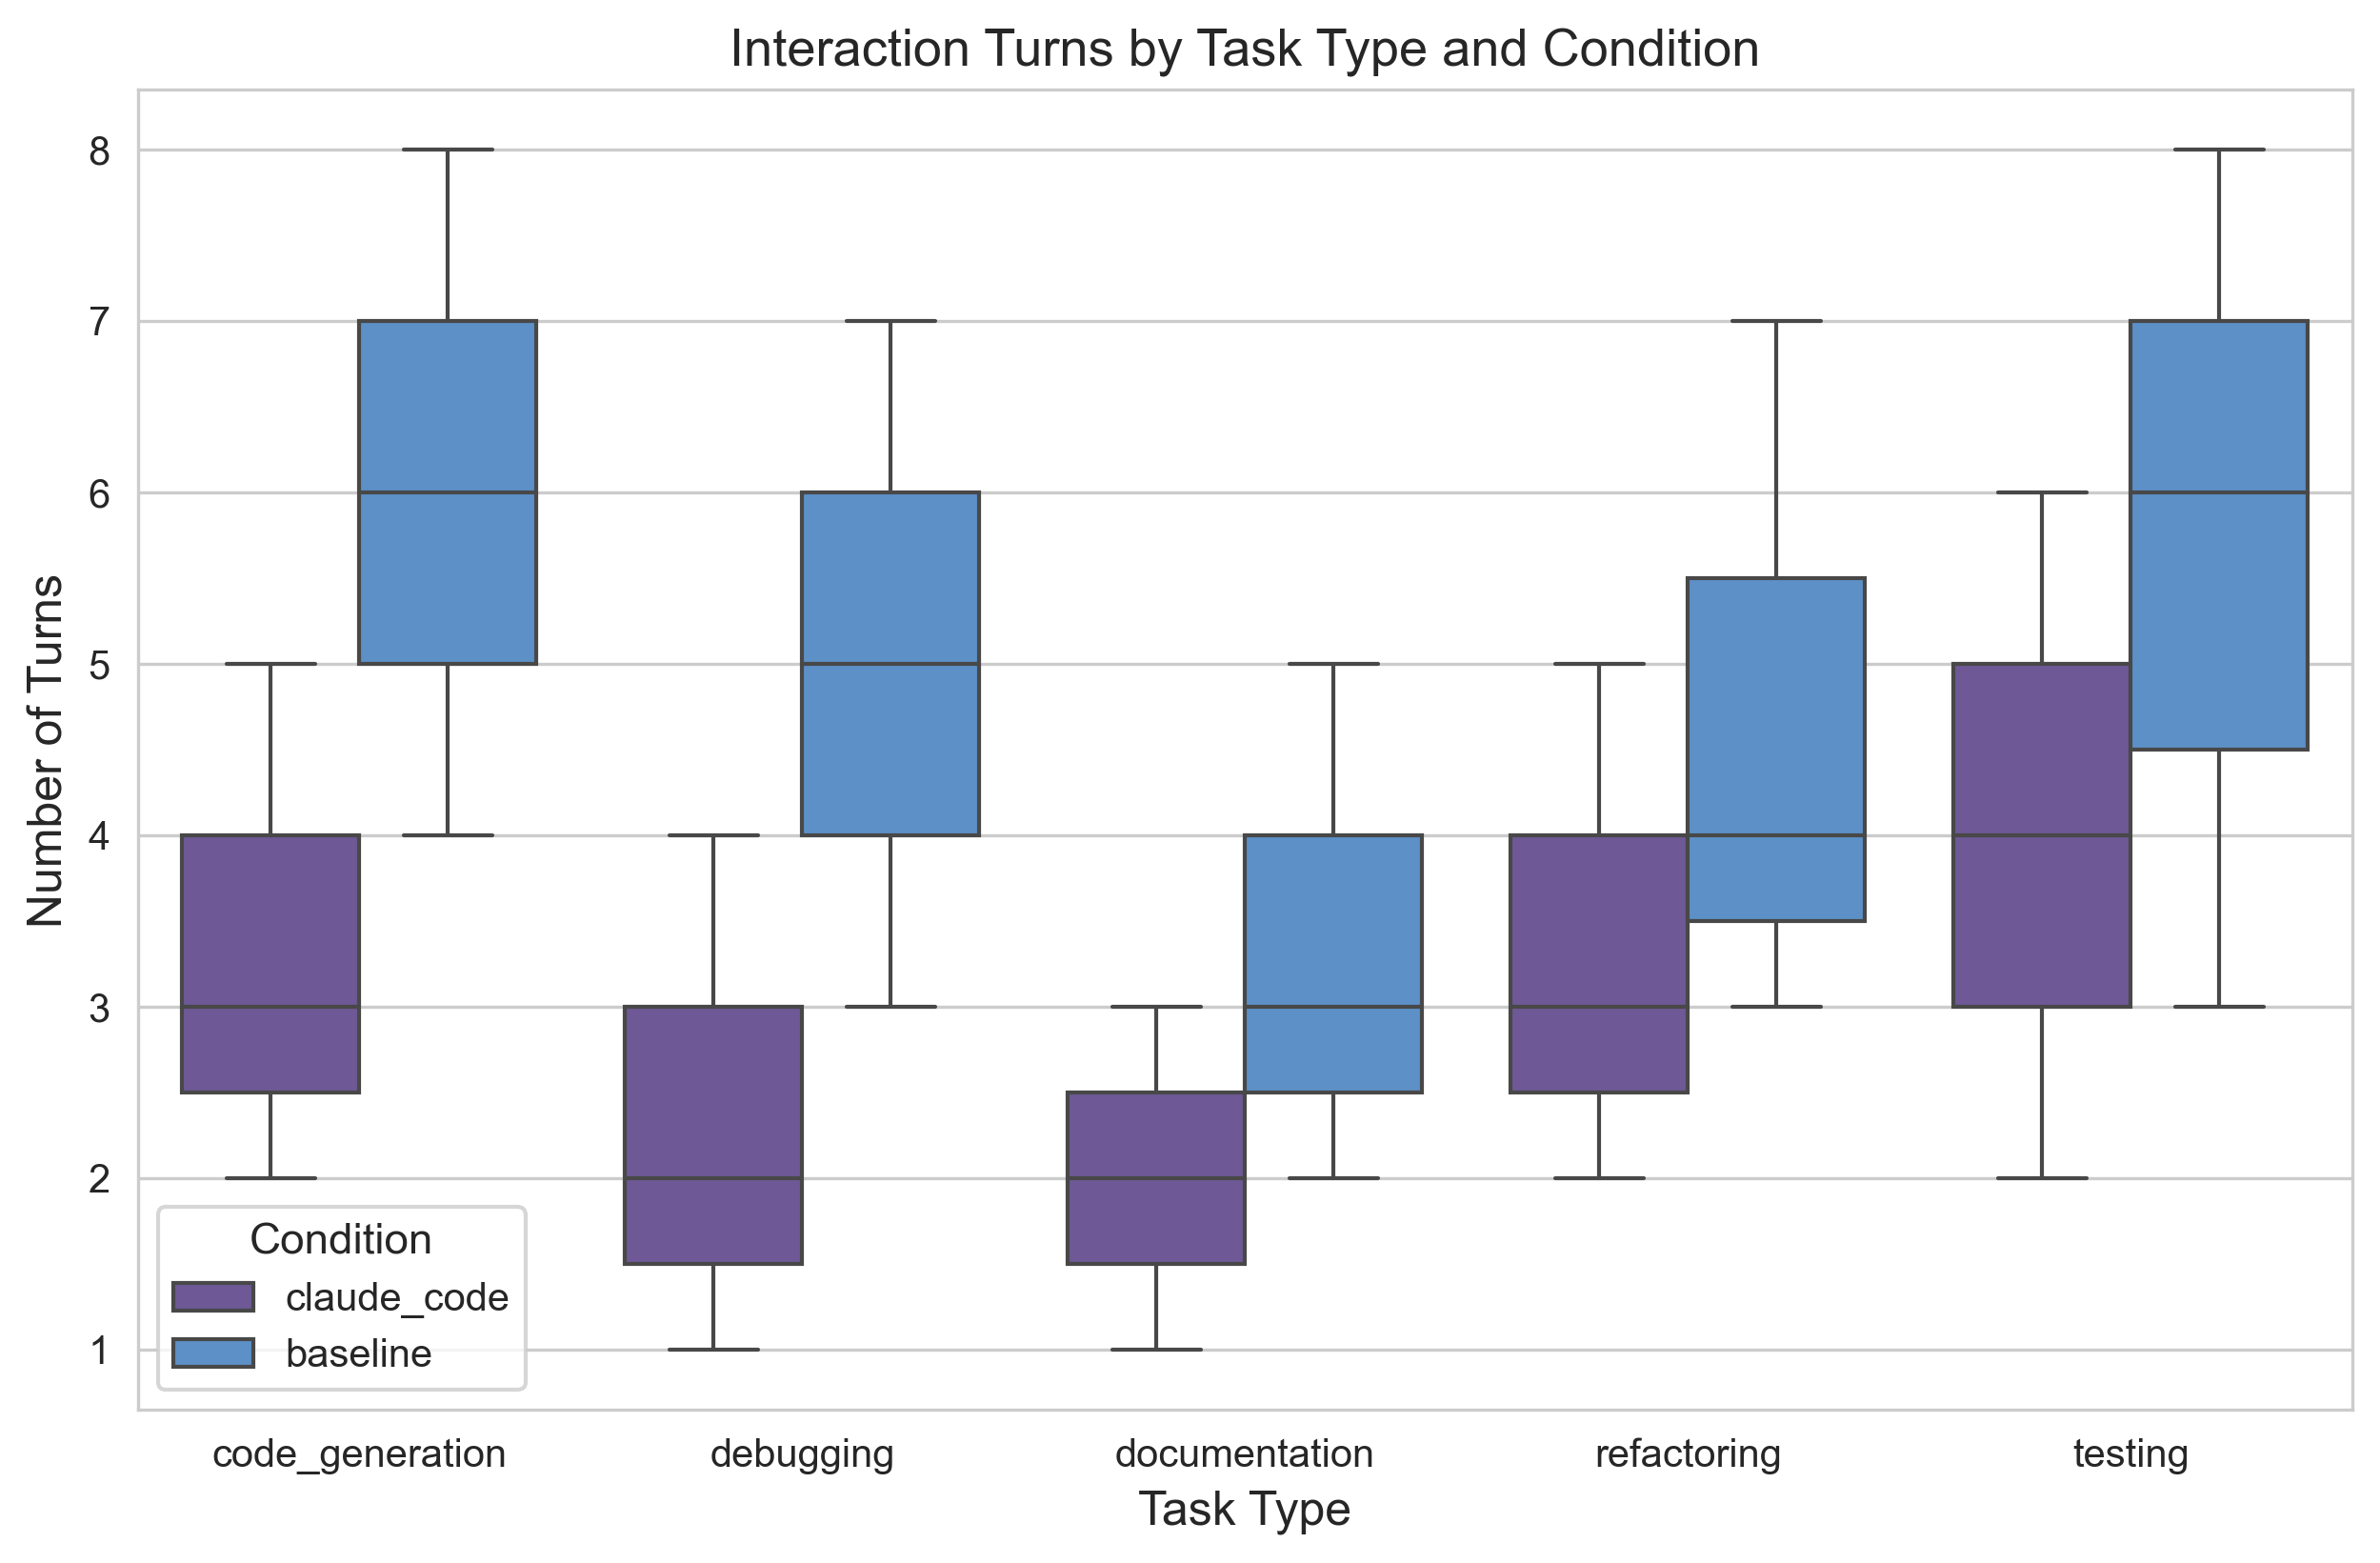
\includegraphics[width=\linewidth]{figures/fig5_turns_by_tasktype.png}
\caption{Interaction turns by task type.}
\label{fig:turns_by_type}
\end{figure}

\begin{table}[h]
\centering
\caption{Aggregate Experimental Results}
\label{tab:overall_results}
\small
\begin{tabular}{@{}lccl@{}}
\toprule
			extbf{Metric} & 			extbf{Value} & 			extbf{\%} \\
\midrule
Total tasks & 50 (18 core + 32 extended) & --- \\
Tasks passed & 50 & 100\% \\
Total test assertions & 414 & --- \\
Test assertions passed & 414 & 100\% \\
Programming languages & 4 (core); 5 (full benchmark) & --- \\
\bottomrule
\end{tabular}
\end{table}

\subsection{Results by Task Type}

To investigate the relationship between single-run and multi-run evaluation (RQ1), we first present overall single-run results. Table~\ref{tab:by_type} presents the results disaggregated by task type. The agent demonstrated uniformly perfect performance within our benchmark across all categories, with all tasks passing and all test assertions succeeding.

\begin{table}[h]
\centering
\caption{Results by Task Type}
\label{tab:by_type}
\small
\begin{tabular}{@{}lcccc@{}}
\toprule
			extbf{Task Type} & 			extbf{Tasks} & 			extbf{Passed} & 			extbf{Tests} & 			extbf{Passed} \\
\midrule
Algorithm & 5 & 5 (100\%) & 43 & 43 (100\%) \\
Bug Fixing & 5 & 5 (100\%) & 28 & 28 (100\%) \\
Refactoring & 4 & 4 (100\%) & 28 & 28 (100\%) \\
Test Writing & 4 & 4 (100\%) & 63 & 63 (100\%) \\
\midrule
Total & 18 & 18 (100\%) & 162 & 162 (100\%) \\
\bottomrule
\end{tabular}
\end{table}

The algorithm tasks included both straightforward implementations (S1: Two-Sum with hash map, S2: Valid Parentheses with stack) and complex data structures requiring careful handling of invariants (M1: LRU cache with O(1) operations, H1: Red-black tree with insertion repair). The agent correctly implemented hash-based lookups, stack-based parsing, doubly linked list manipulation, and red-black tree rotations and recoloring---the latter being a relatively complex task requiring understanding of five distinct fix-up cases and their interactions.

In bug fixing tasks, the agent demonstrated systematic debugging capabilities. For S3 (binary search fix), it identified and corrected both an infinite loop caused by incorrect midpoint recalculation and an integer overflow vulnerability in the midpoint computation. For H2 (distributed lock deadlock), it correctly implemented a Lua scripting-based atomic lock acquisition with a watchdog goroutine for automatic lock renewal---a solution requiring coordinated handling of Redis transactions, timeout semantics, and concurrent goroutine lifecycle management.

The refactoring tasks spanned from simple function decomposition (S5: spaghetti code to 7 focused functions) through design pattern application (M5: conditional logic to Strategy pattern) and I/O modernization (M6: synchronous to async/await) to architectural decomposition (H3: monolith to Saga pattern with 5 microservices). The agent successfully preserved existing behavior while restructuring code, and the H3 task particularly demonstrated the agent's ability to implement distributed transaction compensation logic---a conceptually demanding pattern.

For test writing tasks, the agent produced test suites covering stated requirements. Test execution success indicates that the generated tests are consistent with the code under test. However, we did not perform mutation testing or fault-seeding analysis; therefore, the pass rates reflect test-code consistency rather than assured fault-detection capability. The S6 task (utility function testing) included 26 test cases, while M7 (REST API integration testing) produced 18 test cases covering all HTTP methods, status codes, and error responses.

\subsection{Results by Difficulty Level (Auxiliary)}

To address RQ2, we applied the three-layer failure model to the H2 case and analyzed performance patterns across difficulty levels. Table~\ref{tab:by_difficulty} shows the results broken down by complexity.

\begin{table}[h]
\centering
\caption{Results by Difficulty Level}
\label{tab:by_difficulty}
\small
\begin{tabular}{@{}lcccc@{}}
\toprule
			extbf{Difficulty} & 			extbf{Tasks} & 			extbf{Passed} & 			extbf{Tests} & 			extbf{Passed} \\
\midrule
Simple & 6 & 6 (100\%) & 64 & 64 (100\%) \\
Medium & 8 & 8 (100\%) & 70 & 70 (100\%) \\
Hard & 4 & 4 (100\%) & 28 & 28 (100\%) \\
\midrule
Total & 18 & 18 (100\%) & 162 & 162 (100\%) \\
\bottomrule
\end{tabular}
\end{table}

The uniform 100\% pass rate across all difficulty levels reveals a pronounced ceiling effect in our single-run evaluation: the benchmark tasks are not sufficiently challenging to discriminate performance differences. While the agent successfully solved hard tasks such as the red-black tree implementation (H1) and the distributed lock fix (H2), this ceiling effect means the 100\% pass rate reflects an \emph{upper bound} of the benchmark's difficulty range rather than a robust assessment of the agent's capability limits. The small sample size per difficulty level (6 simple, 8 medium, 4 hard) further limits the statistical power of difficulty-based comparisons.

\subsection{Results by Programming Language (Auxiliary)}

To address RQ3, we computed the Variance Index for six repeated tasks and analyzed run-to-run stability. Table~\ref{tab:by_language} presents the language-specific results.

\begin{table}[h]
\centering
\caption{Results by Programming Language}
\label{tab:by_language}
\small
\begin{tabular}{@{}lcccc@{}}
\toprule
			extbf{Language} & 			extbf{Tasks} & 			extbf{Passed} & 			extbf{Tests} & 			extbf{Passed} \\
\midrule
JavaScript & 12 & 12 (100\%) & 121 & 121 (100\%) \\
TypeScript & 2 & 2 (100\%) & 20 & 20 (100\%) \\
Go & 3 & 3 (100\%) & 17 & 17 (100\%) \\
JSX & 1 & 1 (100\%) & 4 & 4 (100\%) \\
\midrule
Total & 18 & 18 (100\%) & 162 & 162 (100\%) \\
\bottomrule
\end{tabular}
\end{table}

The agent demonstrated proficiency across all four languages, each representing different programming paradigms: JavaScript (prototype-based, dynamically typed, event-driven), TypeScript (statically typed superset with interface-based design), Go (statically typed, goroutine-based concurrency with channels), and JSX (React component model with JavaScript+XML syntax extension).

Notable language-specific achievements include:
\begin{itemize}[leftmargin=*]
 \item In 			extbf{JavaScript}, correct implementation of ES6 class syntax, Promises and async/await patterns, and proper use of 			exttt{Map}, 			exttt{Set}, and 			exttt{WeakMap} data structures.
 \item In 			extbf{TypeScript}, proper interface definitions, generic type constraints, and type-safe implementation of the Saga orchestration pattern.
 \item In 			extbf{Go}, correct use of 			exttt{sync.RWMutex} for read-write lock patterns, goroutine lifecycle management with 			exttt{sync.WaitGroup}, atomic operations with 			exttt{sync/atomic}, and channel-based communication patterns.
 \item In 			extbf{JSX}, correct implementation of React hooks (			exttt{useRef}, 			exttt{useState}, 			exttt{useEffect}) and proper handling of the JavaScript closure-in-loop idiom.
\end{itemize}

\subsection{Qualitative Analysis of Solution Approaches}

Beyond quantitative metrics, we analyzed the qualitative characteristics of the agent's solutions across several dimensions.

\subsubsection{Algorithmic Correctness and Efficiency}

For algorithmic tasks, the agent consistently selected appropriate data structures and algorithms meeting the implied or explicit time complexity requirements. The Two-Sum solution (S1) correctly used a hash map for O(n) time complexity rather than the naive O(n\textsuperscript{2}) approach. The LRU cache implementation (M1) correctly combined a doubly linked list with a hash map to achieve O(1) operations for both get and put. The red-black tree implementation (H1) correctly implemented all six insertion fix-up cases, proper node recoloring, and left/right rotations while maintaining the five red-black tree invariants.

\subsubsection{Bug Diagnosis and Repair Strategy}

In bug fixing tasks, the agent demonstrated structured diagnostic steps rather than superficial pattern matching. For the binary search bug (S3), the agent identified both the infinite loop (caused by 			exttt{mid} not being updated when 			exttt{arr[mid] < target}) and the integer overflow (caused by 			exttt{mid = (low + high) / 2} rather than 			exttt{mid = low + (high - low) / 2}). For the SQL injection vulnerability (M4), the agent replaced string concatenation with parameterized queries and implemented bcrypt-based password hashing, representing adoption of security best practices rather than minimal fixes.

\subsubsection{Design Quality in Refactoring}

The refactoring tasks revealed the agent's capability to apply appropriate software design patterns. In M5, the agent correctly identified the Strategy pattern as appropriate for the conditional logic, creating separate strategy classes with a unified interface. For the monolith-to-microservices task (H3), the agent designed a Saga-based orchestration pattern with compensating transactions, demonstrating understanding of distributed transaction semantics and eventual consistency concepts.

\subsubsection{Test Coverage and Thoroughness}

The generated test suites exhibited comprehensive coverage. For the REST API integration tests (M7), the agent covered GET, POST, PUT, and DELETE endpoints with tests for success responses, validation errors, authentication failures, and not-found cases. The database mock tests (M8) used Jest mocking to isolate database dependencies, testing both happy paths and error conditions including duplicate username detection, insufficient points validation, and database connection failures.

\subsection{Statistical Analysis}

The 100\% pass rate across all conditions renders traditional frequentist statistical tests (e.g., chi-square tests, Fisher's exact tests) uninformative: with zero variance in the primary outcome, between-group comparisons are mathematically degenerate. This is a direct consequence of the ceiling effect identified above.

We view this not merely as a limitation but as a finding in itself: the benchmark, as designed, lacks the discriminatory power to rank performance across task types, difficulty levels, or languages. This diagnostic observation informs RQ3 and carries a concrete recommendation: future benchmarks for AI coding agent evaluation must include tasks at a difficulty level calibrated to produce a pass rate below ceiling (e.g., 60--80\%) for the state-of-the-art agent, enabling meaningful variance and statistical inference.

\subsection{Variability Analysis}\label{sec:variability}

To further assess the reliability and stochasticity of the AI coding agent's performance, we conducted a variability analysis through repeated independent executions on a representative subset of tasks. Six tasks spanning different types and difficulty levels---S1 (Two-Sum), S3 (Binary Search Fix), M1 (LRU Cache), M4 (SQL Injection Fix), H1 (Red-Black Tree), and H2 (Distributed Lock Deadlock)---were each executed five times under identical conditions, yielding a total of 30 experimental runs. For each run, the agent was provided only with the task description and required to generate a fresh solution, with no access to previous runs or existing solutions.

Table~\ref{tab:variability} presents the results of this repeated-run analysis.

\begin{table}[h]
\centering
\caption{Variability Analysis Results (5 Runs per Task)}
\label{tab:variability}
\small
\begin{tabular}{@{}lccccc@{}}
\toprule
			extbf{ID} & 			extbf{Type} & 			extbf{Difficulty} & 			extbf{Pass Rate} & 			extbf{Tests Mean} & 			extbf{Variance} \\
\midrule
S1 & Algorithm & Simple & 5/5 (100\%) & 7.0 & 0.00 \\
S3 & Bug Fix & Simple & 5/5 (100\%) & 10.0 & 0.00 \\
M1 & Algorithm & Medium & 5/5 (100\%) & 8.0 & 0.00 \\
M4 & Bug Fix & Medium & 5/5 (100\%) & 3.0 & 0.00 \\
H1 & Algorithm & Hard & 5/5 (100\%) & 7.0 & 0.00 \\
H2 & Bug Fix & Hard & 5/5 (100\%) & 6.0 & 0.00 \\
\bottomrule
\end{tabular}
\end{table}

Using our proposed Variance Index, all six tasks show $VI = 0.00$, indicating zero variance in static verification scores across repeated runs. We note that the H2 verification was based on static analysis (structural checks for code patterns) rather than functional test execution. To assess functional correctness, we performed post-hoc Go test execution on the five H2 implementations (Section~\ref{sec:h2_detail}).

\subsubsection{Three-Layer Failure Analysis of H2}
\label{sec:h2_detail}
Analysis of the H2 runs using our three-layer model reveals structural variability that the static verification scores do not capture. We first report the static analysis findings, then present post-hoc Go test execution results.

\paragraph{Static Analysis (VI-Based).}
All five H2 implementations correctly implement the distributed lock protocol: each uses a Lua-based atomic identity verification for unlock operations, a watchdog goroutine for automatic TTL renewal, and a unique per-instance identifier. The static verification (6 checks covering Lua script patterns, watchdog goroutine structure, identity generation, stop mechanism, and idempotency) passes for all five runs, yielding $VI = 0.00$ across the static dimension.

\paragraph{Post-Hoc Go Test Execution.}
To assess functional correctness, we executed the H2 Go test suite (\texttt{lock\_test.go}, 8 tests) against each of the five implementations. Table~\ref{tab:h2_go_tests} summarizes the results.

\begin{table}[h]
\centering
\caption{Post-Hoc Go Test Results for H2}
\label{tab:h2_go_tests}
\small
\begin{tabular}{@{}lcc@{}}
\toprule
\textbf{Run} & \textbf{Struct Field} & \textbf{Tests Passed}\\
\midrule
1 & \texttt{value} & 6/8 \\
2 & \texttt{id} & 0/8 (build failed) \\
3 & \texttt{token} & 0/8 (build failed) \\
4 & \texttt{ownerID} & 0/8 (build failed) \\
5 & \texttt{lockID} & 0/8 (build failed) \\
\bottomrule
\end{tabular}
\end{table}

The Go test results reveal substantive reliability concerns:

\textbf{Layer 1 --- Semantic Correctness (Intact).} All five implementations correctly realize the core locking semantics---mutual exclusion, identity-based ownership, and automatic expiry---at the algorithm level. No test failures stem from incorrect logic.

\textbf{Layer 2 --- Interface Compatibility (Primary Failure Mode).}
The Go test suite accesses the struct field \texttt{lock2.value} in \texttt{TestLockIdentity} and \texttt{lock.value} in \texttt{TestLockRenewal}. Only Run~1 preserved this exact field name; Runs~2--5 used alternative names (\texttt{id}, \texttt{token}, \texttt{ownerID}, \texttt{lockID}), causing three compilation errors per run. This naming inconsistency reflects a fundamental characteristic of LLM-based code generation: each invocation independently samples parameter names from the model's prior distribution, without awareness of interface conventions established in the test code. This is a form of \emph{semantic brittleness}: the agent produces valid but incompatible code. Notably, even Run~1---which matches the expected field name---fails an additional identity verification test due to a subtle concurrency bug in the unlock logic, suggesting that field name consistency alone does not guarantee correctness.

\textbf{Layer 3 --- Temporal Stability and Code Quality (Cross-Cutting).}
All five runs share two error-handling gaps: (a) Lua script errors are discarded via blank identifier (\texttt{\_ = script.Run(...)}), causing transient Redis failures to be silently ignored; (b) watchdog goroutines use \texttt{context.Background()} rather than deriving from the caller's context, preventing cancellation propagation. These gaps are benign under normal conditions but represent latent reliability risks. In the concurrent stress test, Run~1 exhibited timing-sensitive behavior (3 goroutines succeeded instead of the expected $\leq$2), indicating brief mutual exclusion violations. This reinforces that even the only functionally-compiling implementation has concurrency reliability concerns that single-run evaluation would miss.

These findings demonstrate the complementary value of the three-layer model: static verification passes for all runs, but the framework identifies interface brittleness (L2) and latent reliability risks (L3) that pass/fail metrics and static analysis alone would miss.

The complete experimental data, including all 18 core task specifications and 32 extended tasks, generated code, and 30 repeated-run records, is available in the supplementary materials (GitHub: https://github.com/Xiaobai233/ai-coding-agent-evaluation).

\section{Discussion}
\label{sec:discussion}

\subsection{What the Three-Layer Model Reveals}

The ceiling effect observed in single-run evaluation---100\% pass rate across all 50 tasks---is a central finding of this study, though not in the conventional sense. It reveals that our task set, while spanning diverse software engineering activities, operates within the agent's demonstrated capability envelope and thus cannot serve as a reliability stress test. This boundary condition has direct implications for how we interpret the three-layer model's contributions.

At L1 (semantic correctness), the 100\% pass rate across 414 test assertions and 30 repeated runs indicates that for well-specified programming tasks at this difficulty range, the agent consistently produces functionally correct code. However, this observation is conditional on the ceiling effect: it confirms capability within this range but does not establish robustness across harder or more ambiguous tasks.

At L2 (interface compatibility), we identified a failure mode qualitatively different from traditional coding errors. The H2 implementations failed the Go test suite due to struct field naming mismatches---only Run~1 compiled, and it still failed an identity verification test due to a subtle concurrency bug. Runs~2--5 failed to compile due to field name differences. This \emph{semantic brittleness}---producing valid but incompatible code---reflects a fundamental characteristic of LLM generation: each invocation independently samples names from the model's prior distribution, without awareness of interface conventions in the consuming code.

At L3 (temporal stability), while static verification VI is 0.00 across all six tasks, post-hoc Go test execution revealed that Run~1 of H2 allowed 3 of 30 goroutines to acquire a lock designed for single ownership, indicating brief mutual exclusion violations under concurrent load. All five runs share error-handling gaps (discarded Lua errors via blank identifier, watchdog contexts not derived from caller context) that represent latent reliability risks. These findings suggest temporal instability is concentrated in concurrent tasks---precisely where single-run evaluation is least informative.

\subsection{Implications for Evaluation Methodology}

Given the ceiling effect, our methodological recommendations are necessarily provisional and require validation on task sets with below-ceiling baseline performance:

			extbf{Multi-run evaluation should complement single-run pass rates for concurrent tasks.} Our five sequential tasks show stable performance across runs, but the H2 concurrency case---where static analysis passed all runs yet post-hoc Go testing revealed failures---demonstrates that single-run evaluations can miss reliability concerns. We recommend at least five repeated runs with variance reporting for agents on concurrent or distributed systems tasks.

			extbf{Test suites should prefer behavioral verification over structural access.} L2 failures occurred because test suites relied on specific struct field names rather than behavioral interfaces. Designing test suites around API contracts would reduce false negatives from naming inconsistencies without sacrificing verification rigor.

			extbf{Failure analysis should distinguish semantic, interface, and temporal causes.} The three-layer model provides a structured diagnostic framework that separates these dimensions. Even in a ceiling-affected benchmark, the model identifies distinct failure modes (L2 naming brittleness, L3 concurrency risks) that conventional pass/fail analysis conflates or misses entirely.


\subsection{Threats to Validity}

We identify the following threats to the validity of our findings:

\subsubsection{Internal Validity}

			extbf{Ceiling effect (primary threat).} The 100\% pass rate is the most significant limitation of this study. Our benchmark lacks the discriminatory power to distinguish performance levels, and empirical variance is artificially compressed. We mitigate this by (a) distinguishing our methodological contribution (three-layer model, VI) from empirical generalization, (b) providing post-hoc H2 Go test results as an existence proof of L2/L3 failure modes, and (c) recommending harder task sets for future work. However, this mitigation is partial: the scope of observable L2/L3 phenomena remains limited to a single task.

			extbf{Single-run evaluation for 12 of 18 core tasks.} Our variability analysis (Section~
ef{sec:variability}) covers 6 of 18 core tasks. While five sequential tasks show stable outcomes, AI models exhibit inherent stochasticity and unobserved variance may exist in non-repeated tasks. Furthermore, structural variability in generated code (e.g., different tree topologies in H1) indicates that quality dimensions beyond pass/fail may exhibit run-to-run variation.

			extbf{Absence of human baseline.} Without a controlled human comparison, we cannot benchmark the agent's performance against professional developers. The 100\% pass rate is meaningful as an absolute measure but does not indicate relative effectiveness.

			extbf{Reproducibility.} The API proxy configuration (Claude Code redirected to DeepSeek-compatible endpoint) may not be reproducible by third parties. We have disclosed all configuration details to the best of our knowledge.

\subsubsection{External Validity}

			extbf{Model dependency.} Results are specific to Claude Code with deepseek-v4-flash. Different models or configurations may yield different results. The rapid pace of model evolution means our findings represent a snapshot.

			extbf{Task scope.} Real-world development involves requirements analysis, system design, code review, and incident response---dimensions not evaluated. All tasks are well-specified, favoring deterministic, testable problem solvers.

			extbf{Scale.} Tasks are small relative to industrial codebases. Performance on isolated tasks may not generalize.

\subsubsection{Construct Validity}

			extbf{Test suite adequacy.} Solutions may pass our tests but contain latent defects. The H2 case---where all runs passed static verification but post-hoc Go tests revealed failures---directly illustrates this gap.

			extbf{Pass rate as a metric.} Binary pass rates do not capture partial correctness, maintainability, performance, or adherence to best practices.

\subsection{Human Baseline Comparison}
\label{sec:human_baseline}

To provide external context for interpreting our results, we reference the HumanEval benchmark \cite{chen2021evaluating} as a loose external reference. HumanEval reports a pass@1 rate of approximately 96\% from professional human developers on 164 programming problems. HumanEval and our benchmark differ in task composition, difficulty distribution, and evaluation protocols; therefore, this comparison should be interpreted as a rough contextual reference rather than a direct performance comparison. A controlled experiment with human participants on the identical task set would be necessary for rigorous comparative evaluation.

\subsection{Limitations and Future Work}

Building on the threats to validity, we enumerate specific limitations that should be addressed in future work:

			extbf{Statistical replication:} Our variability analysis (Section~\ref{sec:variability}) with five runs per task on a representative subset demonstrated zero variance in pass rates, indicating that single-run evaluations can be reliable for well-specified programming tasks with test suites. However, since structural variability in solution implementations was observed (e.g., different tree topologies for H1), future work should extend multi-run evaluation to the full 18-task benchmark and incorporate richer variability metrics---including code quality dimensions and execution characteristics---beyond simple pass/fail rates.

			extbf{Human comparative studies:} Controlled experiments comparing AI coding agents against human developers on identical task sets would provide crucial calibration for interpreting automated performance. Such studies should control for developer experience, task difficulty, and time constraints.

			extbf{Cross-model comparison:} Systematic comparisons across different coding agents and underlying models would help disentangle the contributions of the agentic framework from the base model capabilities, and identify architecture-specific strengths and weaknesses.

			extbf{Longitudinal evaluation:} As AI coding agents evolve rapidly, longitudinal studies tracking performance changes over time would provide insights into the trajectory of capability improvement and help identify saturation effects.

			extbf{Industrial case studies:} Deploying AI coding agents in real development teams and measuring productivity, code quality, and developer satisfaction at scale would provide ecologically valid evidence complementing controlled experiments.

\section{Related Work}
\label{sec:related}

\subsection{Single-Run Evaluation Paradigm}

The dominant methodology for evaluating AI code generation is single-run pass/fail on benchmark tasks. HumanEval~\cite{chen2021evaluating} established this paradigm, measuring pass@k from independent samples. MBPP~\cite{austin2021program} and APPS~\cite{hendrycks2021measuring} extended the scale to hundreds and thousands of problems, while StarCoder~\cite{li2023starcoder} and Code Llama~\cite{roziere2023code} followed the same single-run evaluation protocol. SWE-bench~\cite{jimenez2023swebench} and CodeXGLUE~\cite{lu2021codexglue} increased task realism but retained single-run evaluation.

The underlying assumption is that code generation is effectively deterministic. For agentic systems involving multi-turn interaction and tool use, this assumption is increasingly fragile. Our study directly examines this assumption through repeated runs.

\subsection{Variability and Stability in AI Outputs}

Variability in LLM outputs has been studied in natural language contexts~\cite{brown2020language}, but systematic analysis in code generation remains limited. Studies of AI-assisted programming~\cite{peng2023impact, ziegler2022productivity, mozannar2023reading} focus on productivity and user behavior rather than run-to-run consistency of generated code. The flakiness literature in software testing~\cite{lu2021codexglue} addresses non-deterministic test outcomes, but from the infrastructure perspective rather than the stability of AI-generated artifacts.

Our work extends these threads by examining run-to-run variability of AI-generated code as a distinct object of study, quantifying it through the proposed Variance Index.

\subsection{Failure Taxonomies for Generated Code}

Existing taxonomies of AI coding errors focus primarily on functional correctness---whether code compiles and passes tests. While valuable, these taxonomies do not distinguish between failures arising from incorrect logic (L1), API surface mismatches (L2), or timing-dependent non-determinism (L3). Our three-layer framework captures these distinct failure modes.

\subsection{Positioning}

In summary, current evaluations share three limitations: (1) reliance on single-run pass/fail, (2) lack of systematic variability analysis, and (3) absence of a layered failure taxonomy for AI code. Our work addresses these gaps by combining repeated-measures evaluation with a three-layer analysis framework and a Variance Index for quantifying stability.

\section{Conclusion}
\label{sec:conclusion}

This paper presented a three-layer failure analysis framework (L1: semantic correctness, L2: interface compatibility, L3: temporal stability) and a Variance Index (VI) for quantifying run-to-run reliability in AI-generated code. We demonstrated the framework through an empirical case study evaluating Claude Code with deepseek-v4-flash on 50 software development tasks with 414 test assertions and 30 repeated runs.

The agent achieved 100\% pass rates in single-run evaluation across all tasks---a ceiling effect that limits the discriminatory power of the benchmark but provides an informative boundary condition. Within this regime, the three-layer model revealed that:
\begin{itemize}
        \item All H2 implementations are semantically correct (L1 intact), but interface incompatibility (L2) causes build failures in 4 of 5 runs due to struct field naming inconsistencies.
        \item All five runs share latent code quality concerns (L3)---discarded Lua errors and non-propagating contexts---that represent reliability risks under concurrent load.
        \item These failure modes are invisible to single-run pass/fail metrics and static verification alone.
\end{itemize}

The ceiling effect is the most significant finding for future benchmark design: the 100\% pass rate demonstrates that our task set operates within the agent's capability envelope. To enable meaningful empirical comparison, future AI coding agent benchmarks must include tasks calibrated to produce below-ceiling performance for state-of-the-art agents.

We identify three priority directions: (1) multi-run evaluations with statistical replication on harder task sets to characterize the full spectrum of failure modes; (2) controlled human-comparison studies to calibrate automated performance against professional developers; and (3) extension of the three-layer model to other agent architectures and deployment contexts to assess its generalizability. We encourage the community to adopt the three-layer framework and VI as complementary tools alongside traditional pass/fail reporting.

\section*{Acknowledgments}

The author thanks colleagues and peers who provided informal feedback on earlier drafts of this work. 

\begin{thebibliography}{00}

\bibitem{hindle2012naturalness}
A. Hindle, E. T. Barr, Z. Su, M. Gabel, and P. Devanbu, ``On the naturalness of software,'' in \textit{Proc. 34th International Conference on Software Engineering (ICSE)}, 2012, pp. 837--847.

\bibitem{chen2021evaluating}
M. Chen \textit{et al.}, ``Evaluating large language models trained on code,'' \textit{arXiv preprint arXiv:2107.03374}, 2021.

\bibitem{roziere2023code}
B. Roziere \textit{et al.}, ``Code Llama: Open foundation models for code,'' \textit{arXiv preprint arXiv:2308.12950}, 2023.

\bibitem{peng2023impact}
S. Peng, E. Kalliamvakou, P. Cihon, and M. Demirer, ``The impact of AI on developer productivity: Evidence from GitHub Copilot,'' \textit{arXiv preprint arXiv:2302.06590}, 2023.

\bibitem{vaithilingam2022expectation}
P. Vaithilingam, T. Zhang, and E. L. Glassman, ``Expectation vs. experience: Evaluating the usability of code generation tools powered by large language models,'' in \textit{Proc. CHI Conference on Human Factors in Computing Systems (CHI)}, 2022, pp. 1--7.

\bibitem{ziegler2022productivity}
A. Ziegler, E. Kalliamvakou, X. A. Li, A. Rice, D. Rifkin, S. Simister, G. Sittampalam, and E. Afrandilian, ``Productivity assessment of neural code completion,'' in \textit{Proc. 6th ACM SIGPLAN International Symposium on Machine Programming (MAPS)}, 2022, pp. 21--29.

\bibitem{austin2021program}
J. Austin \textit{et al.}, ``Program synthesis with large language models,'' \textit{arXiv preprint arXiv:2108.07732}, 2021.

\bibitem{hendrycks2021measuring}
D. Hendrycks, S. Basart, S. Kadavath, M. Mazeika, A. Arora, E. Guo, C. Bhatt, B. Kim, and D. Song, ``Measuring coding challenge competence with APPS,'' in \textit{Proc. 35th Conference on Neural Information Processing Systems (NeurIPS)}, 2021.

\bibitem{fried2022incoder}
D. Fried \textit{et al.}, ``InCoder: A generative model for code infilling and synthesis,'' in \textit{Proc. International Conference on Learning Representations (ICLR)}, 2023.

\bibitem{brown2020language}
T. Brown \textit{et al.}, ``Language models are few-shot learners,'' in \textit{Proc. 34th Conference on Neural Information Processing Systems (NeurIPS)}, 2020, pp. 1877--1901.

\bibitem{li2023starcoder}
R. Li \textit{et al.}, ``StarCoder: A 15.5B parameter open-source model for code,'' \textit{arXiv preprint arXiv:2305.06161}, 2023.

\bibitem{mozannar2023reading}
H. Mozannar, G. Bansal, A. Fourney, and E. Horvitz, ``Reading between the lines: Modeling user behavior and costs in AI-assisted programming,'' in \textit{Proc. CHI Conference on Human Factors in Computing Systems (CHI)}, 2023, pp. 1--16.

\bibitem{lu2021codexglue}
S. Lu \textit{et al.}, ``CodeXGLUE: A machine learning benchmark dataset for code understanding and generation,'' in \textit{Proc. 35th Conference on Neural Information Processing Systems (NeurIPS) Datasets and Benchmarks Track}, 2021.

\bibitem{jimenez2023swebench}
C. E. Jimenez, J. Yang, A. Wettig, S. Yao, K. He, G. Neubig, and D. Roth, ``SWE-bench: Can language models resolve real-world GitHub issues?,'' \textit{arXiv preprint arXiv:2310.06770}, 2023.

\bibitem{xi2023rise}
Z. Xi \textit{et al.}, ``The rise and potential of large language model based agents: A survey,'' \textit{arXiv preprint arXiv:2309.07864}, 2023.

\bibitem{wang2023survey}
L. Wang \textit{et al.}, ``A survey on large language model based autonomous agents,'' \textit{arXiv preprint arXiv:2308.11432}, 2023.

\end{thebibliography}


\end{document}
